\documentclass[12pt]{article}

\usepackage{amsfonts,latexsym,amsthm,amssymb,amsmath,amscd,euscript}
\def\arraystretch{1.2}

\usepackage{bold-extra}
\usepackage{framed}
\usepackage{graphicx}
\usepackage[geometry]{ifsym}
\usepackage{hyperref}
\hypersetup{colorlinks=true,citecolor=blue,urlcolor=black,linkbordercolor={1 0 0}}

\textwidth=14.5cm \textheight=20.0cm
\oddsidemargin=1cm
\evensidemargin=1cm

\allowdisplaybreaks[1]
\newcommand\nc{\newcommand}
\nc{\on}{\operatorname}
\nc{\ol}{\overline}

\title{{\textsc{Using Compression to Speed Up Image Classification in Artificial Neural Networks}}}

\author{Dan Fu, Gabriel Guimaraes \\
{\small \texttt{ \{dfu,gabrielguimaraes\}@college.harvard.edu}}}
\date{December 10, 2016}

\begin{document}

\hypersetup{linkcolor = black}

\maketitle

\begin{abstract}
    Traditionally, feature vectors that go into deep learning techniques are easily understandable by humans, but there is nothing inherent to machine learning that makes this a requirement.  We exploit this fact to speed up neural networks by compress image data with an algorithm based on the discrete cosine transform before feeding it to the networks.  We find that we can achieve speedups in training time ranging from $2$ times to $10$ times, depending on the dataset, with only minor effects on algorithm accuracy.
\end{abstract}

\section{Introduction} \label{introduction}

The standard approach to machine learning is to examine the data, derive feature vectors, and feed these feature vectors as inputs to machine learning algorithms.  These feature vectors are often easily understandable by humans as a result.  However, there is nothing inherent to many machine learning algorithms that makes this a requirement.  Given the same information in two sets of feature vectors, a machine learning algorithm should be able to produce the same result using either set.

On the other hand, the goal of compression is to take information and transform it such that it takes up less space but still holds the same amount of information - in other words, to compress vectors from dimension $D$ to $D' < D$ without losing information.  This suggests a natural pairing between the two.  If we can compress feature vectors without losing information, machine learning algorithms should be able to achieve similar correctness results.  At the same time, since the features are of lower dimension, the algorithms should be able to run faster.

In this paper, we test this hypothesis by using the Discrete Cosine Transform - famous from its historical appearance in JPEG compression \cite{wallace} - to speed up Machine Learning algorithms on images.  Traditionally, most Machine Learning papers focus on improving the accuracy of algorithms, with no regard to training time. Training a state of the art deep convolutional neural network can take days even if we have access to big machine clusters. This paper does not attempt to improve the accuracy of ML techniques. Instead, we study the accuracy/training time trade-off curve - attempting to decrease training time by a lot while still maintaining a reasonable accuracy.  We find that a modified version of the discrete cosine transform (we call it DCT + truncate) is a promising approach that can achieve major speedups -- from $2$ times to $10$ times, depending on the data set -- while having only a minor effect on algorithm accuracy.

The paper is organized as follows: in section $\ref{background}$, we discuss the background necessary to understand our approach.  In section $\ref{algorithm}$, we describe our algorithm.  In section $\ref{results}$, we discuss our experimental setup and our results.  In section $\ref{related}$, we discuss related work.  Finally, we conclude in section $\ref{conclusion}$.

\section{Background: The Discrete Cosine Transform} \label{background}

The discrete cosine transform \cite{ahmed} expresses a series of data points as a sum of cosine functions with different frequencies.  In our paper, we use the two-dimensional DCT-II version of the transform (henceforth referred to as ``the DCT transform".  Given an $N \times M$ matrix $A$, the DCT transform converts it to a matrix $X$, whose elements are given by the following equation:

\[ X_{i,j} = \sum_{n = 0}^{N-1} \sum_{n = 0}^{M-1} A_{n, m} \cos\left[ \frac{\pi}{N} \left( n + \frac{1}{2}\right)i \right] \cos\left[ \frac{\pi}{M} \left( m + \frac{1}{2}\right)j \right]\]

The matrix $X$ produced by the DCT transform has a number of useful properties, but the most relevant for our use is its tendency to group values in the top-left (low row and column indices) corner of $X$.  This is useful for the JPEG compression standard because it makes compression via general compression algorithms easier; after a discretization step, most of the values in the final matrix are $0$ and can be compressed easily.  For our purposes, this grouping puts most of the relevant information into the top-left corner of the transformed matrix.  As a result, we can safely truncate a large of the matrix without sacrificing quality.

\section{Our Algorithm} \label{algorithm}

Our algorithm (we call it "DCT truncate") is a simple preprocessing step that can be dropped into the training pipeline of any Machine Learning algorithm. Suppose the input X is a $K \times K$ grayscale image where each pixel is represented as an 8 bit integer. The following algorithm takes in X and returns a $D \times D$ array such that $D \leq K$

\begin{itemize}
  \item Apply the discrete cosine transform to $X$
  \item Pick the $D^2$ elements present in the top left $D$-sided square of the resulting DCT'd matrix
\end{itemize}

This algorithm can be easily generalized to images with multiple color channels (for example RGB) by applying the procedure to each channel separately. At the end, we simply return the concatenation of the three reduced channels.

\section{Results and Discussion} \label{results}

\subsection{The Data Sets}

We tested the above algorithm on two classic Machine Learning image recognition data sets: CIFAR-10 \cite{krizhevsky} and MNIST \cite{lecun}. The former consists of 32x32 color images from 10 classes, with 6000 images per class. The latter consists of grayscale bitmaps of hand-written digits between 0 and 9.

\subsection{The Neural Network Architecture}

For simplicity, we use the same architecture for both data sets. Also, we needed an architecture where the dimension of the input could be changed easily without any adjustment to the hidden layers. We used a hidden layer of size $K1$ that's fully connected to the input and feeds into a dropout layer, which then feeds into a softmax layer. In the CIFAR-10 case, we used $K1 = 512$ and in the MNIST case we used $K1 = 1024$. However, we found that varying $K1$ did not have a big impact on our results.

Convolutional Neural Networks are ubiquitous in image recognition tasks but we chose not to use them because 1) changing the input dimension of a convolutional network can often demand changes in hidden layers, which breaks the fact that we wish to control for the neural network architecture being used and 2) Convolultional Neural Networks depend on the geometrical properties of the image. Namely they depend on the fact that neighbor pixels are often correlated and exhibit locality properties. Using DCT moves us away from the bitmap geometry, so the input vector doesn't carry the same locality properties.

We did, however, run some tests using Convolutional Neural Networks, since this type of architecture is so important in the context of image recognition. In particular, in a quick test we were able to speed up training by a factor of 10 while decreasing the accuracy from 98\% to 92\% in the MNIST data set.

We believe that a more detailed analysis of DCT in the context of Convolutional Neural Networks is instrumental in order to apply DCT to state of the art Machine Learning algorithms, but such an analysis is outside of the scope of this paper.

\subsection{Environment}

We ran our experiments on a late $2013$ MacBook Pro with a $2.3$ GHz quad-core Intel Core i7 processor.  We used the TensorFlow \cite{tensorflow} framework to run our experiments; this framework takes advantage of processor architecture by running training and evaluation of neural networks as local multi-threaded programs.

\subsection{The Results}

Using the above architecture, we ran DCT truncate as a preprocessing step for various values of $D$ on both datasets.  In order to test the DCT truncate technique proposed by this paper, we benchmarked it against three other types of preprocessing: no preprocessing at all, ``DCT truncate end," and Principal Component Analysis (PCA).  DCT truncate end is the same as our DCT truncate algorithm, except we only keep the features in the bottom-right corner of the matrix.  The results for the MNIST dataset are shown in figure $\ref{fig:mnist}$, and the results for the CIFAR-10 dataset are shown in figure $\ref{fig:cifar}$.  Note that the figures report "Number of features" as opposed to $D$. In the CIFAR-10 case the number of features equals $D \cdot D \cdot 3$; in the MNIST case the number of features equals $D^2$.

\begin{figure}
    \centering
    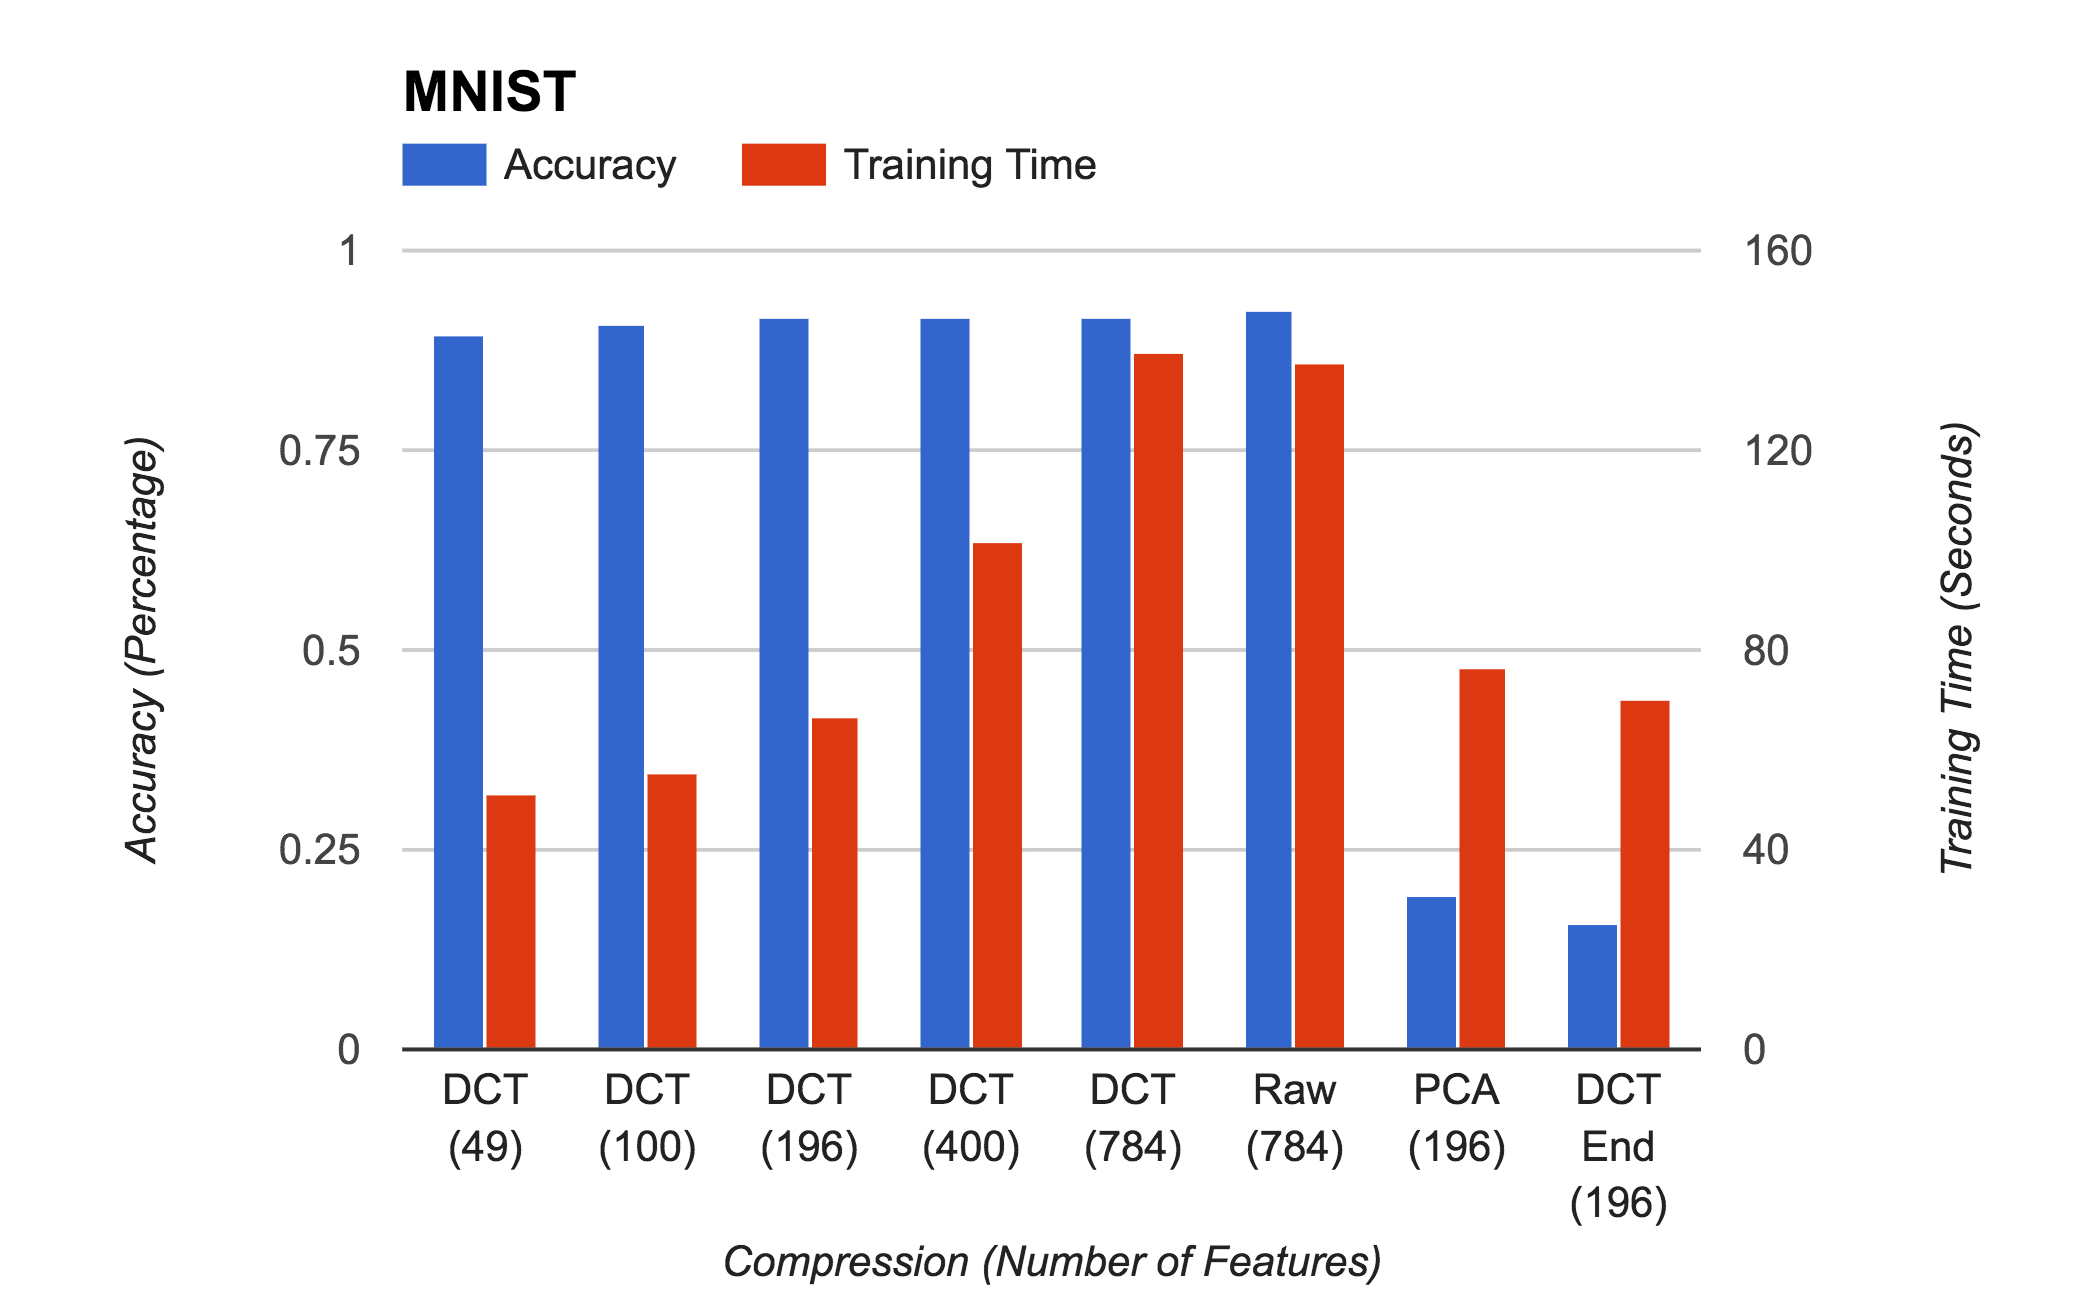
\includegraphics[width=\textwidth]{mnist}
    \caption{Results of our experiments for the MNIST data set.  The DCT columns are our DCT-truncate algorithm, with the number of features left in parentheses.  Raw is the raw image; PCA is the PCA algorithm; and DCT end is DCT, but taking the bottom right corner of the matrix instead of the top left.}
    \label{fig:mnist}
\end{figure}

\begin{figure}
    \centering
    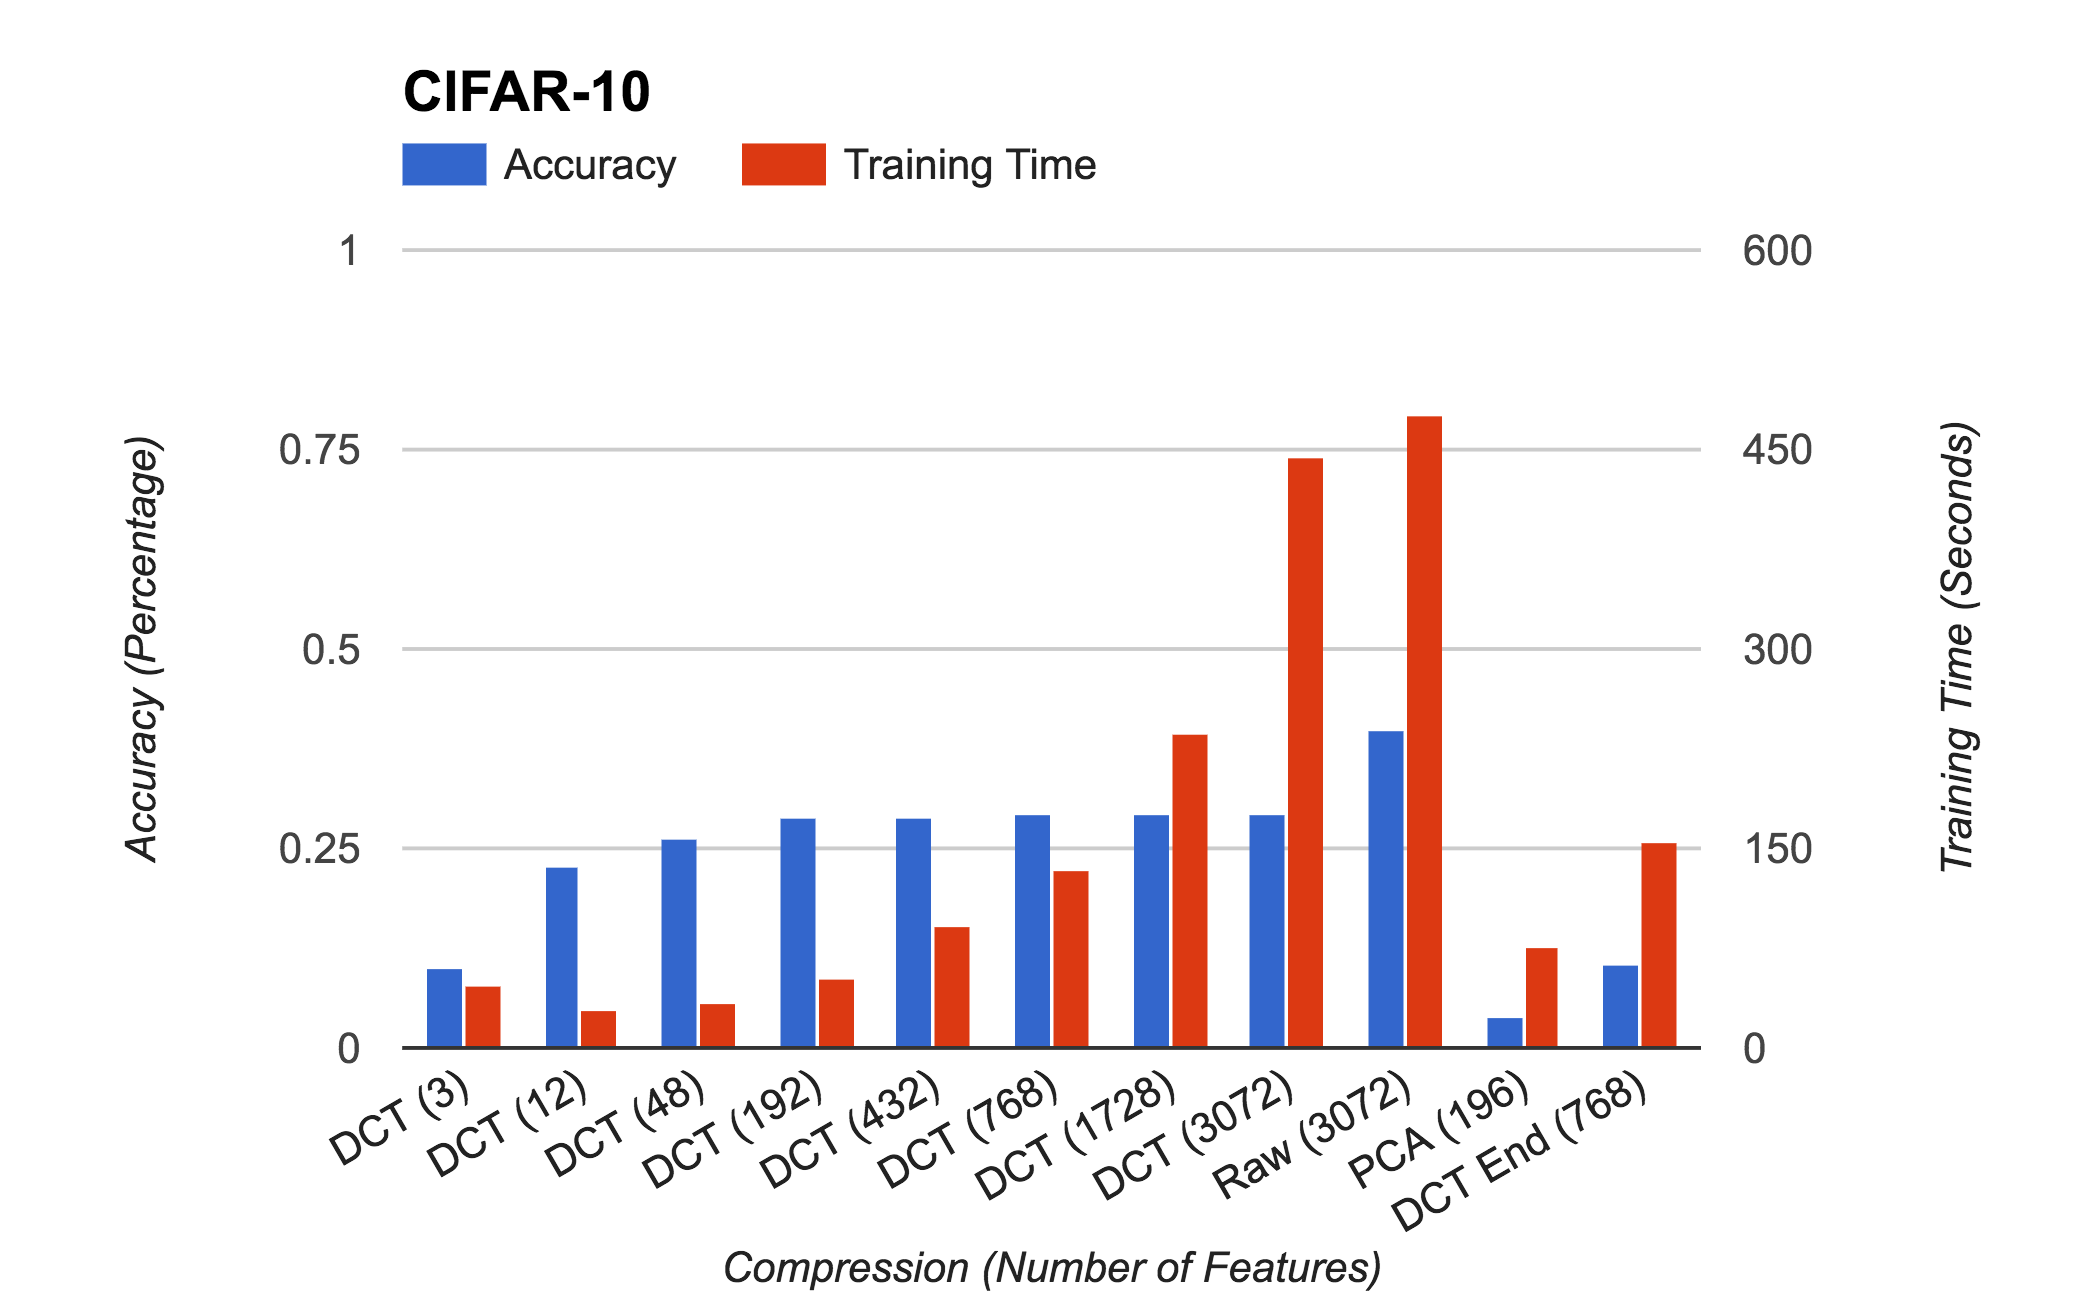
\includegraphics[width=\textwidth]{cifar}
    \caption{Results of our experiments for the CIFAR-10 data set.  The DCT columns are our DCT-truncate algorithm, with the number of features left in parentheses.  Raw is the raw image; PCA is the PCA algorithm; and DCT end is DCT, but taking the bottom right corner of the matrix instead of the top left.}
    \label{fig:cifar}
\end{figure} 

For both datasets, DCT truncate with no truncation and no preprocessing at all performed the same in terms of training time.  However, as we truncated more data, we were able to significantly reduce training time without sacrificing accuracy.  For the MNIST dataset, we were able to reduce the training time by more than half while only sacrificing $1\%$ accuracy.  For the CIFAR-10 dataset, we were able to achieve a $10$-time speedup, but at a $10.92\%$ accuracy hit.  It is interesting to note that this accuracy hit came primarily from the DCT transformation itself and not the truncation; DCT truncate with no truncation performed $10\%$ worse than the raw data.

Looking more closely at the MNIST and CIFAR-10 data it is reasonable to conclude the features that are in the top-left corner of the DCT'ed matrices are the only ones that matter to the machine learning algorithm, since removing them only decreases training time without any measurable effects on accuracy. This is in line with the idea that DCT places almost all of the information in very few features positioned at the top left corner of the resulting matrix.

To test our intuition that only the features in the top-left corner  matter to the ML training, we ran another experiment consisting of truncating the DCT'd matrix but picking features from the bottom right corner, as opposed to the top left corner. These results are displayed in the DCT End column of our figures.  In both MNIST and CIFAR-10 this technique yielded results that are very close to random guessing, which confirms our hypothesis.

\subsection{Principal Component Analysis}

When considering the problem of decreasing the size of input vectors while still preserving entropy, Principal Component Analysis \cite{jolliffe} is one of the first approaches from the Machine Learning literature that comes to mind. By choosing the features with largest eigenvalues in the sample covariance matrix, PCA is able to pick the features with most entropy.

In practice, however, we found that using PCA yielded a model with wild amounts of overfitting. In particular, we tried using PCA to decrease the dimensionality of our data set to the same dimensionality achieved by DCT with little penalty to accuracy. In the CIFAR case, PCA performed worse than random in our test set. In the MNIST case, PCA performed slightly better than random, but much worse than any other technique.

\section{Related Work} \label{related}

There has been some work in the literature on extracting human-readable features from compressed images.  Shen and Sethi \cite{shen} try to extract features such as edges from compressed data.  Likewise, Hafed and Levine \cite{hafed} aim to extract features using the discrete cosine transform.  Our work differs from these two approaches because we are not aiming to extract specific human-readable features from compressed data; in fact, we leverage the insight that finding human-readable features is irrelevant for many machine learning algorithms.

In the field of compressing image feature vectors, Zhang et. al. \cite{zhang16} present the state of the art in compressing high-dimensional feature vectors for image recognition and retrieval.  They compare several methods for compressing high-dimensional feature vectors and argue that feature selection (i.e., reducing the dimensionality of high-dimensional feature vectors instead of explicitly compressing them) is more effective for storing high-dimensional feature vectors.  Their work differs from ours in two crucial ways: first, they start from existing feature vectors, instead of raw bitmaps.  Second, their primary goal is for storage.  As such, some of their techniques may render the data unusable for machine learning.  For example, we strongly suspect that a non-differentiable transformation would make the result unusable for our purposes.  While exploring that hypothesis is outside the scope of this paper, we hope to explore the question in the future.

Moving on to another problem space, Ramaswamy and Gopalakrishnan \cite{ramaswamy} describe a compression algorithm for encoding acoustic features used in speech recognition systems.  This is another direction that we would like to explore in the future, but is also outside the scope of this paper.

We now move on to work related to the use of compression in general feature spaces.  Sculley and Brodley \cite{sculley} use compression on feature vectors as a similarity measure.  Their fundamental idea is that if two string compress more effectively together than they do apart, they must share similar information.  While this insight is not directly applicable to our work, it may inform future attempts to apply our idea to non-image domains.

Hu et. al. \cite{hu} introduce a method for entropy-based feature selection.  They extend Shannon's entropy to a general case and use it to find correlations between different features in a stronger way than the standard approaches using the correlation coefficient.  Zeng et. al. \cite{zeng} augment Hu's work by treating the different feature vectors as cooperators in a game and using methods from game theory and the entropy-based approach to further refine the feature selection approach.  We suspect that both these approaches will be helpful in future attempts to apply our idea to general feature spaces.

\section{Conclusion and Future Work} \label{conclusion}

In this paper we applied the Discrete Cosine Transform from compression theory to reduce the dimensionality of feature vectors, thus speeding up the training of deep neural networks. In our experiments we were able to decrease the training time by up to a factor of 10. However, we saw a decrease in accuracy of the algorithms as expected.

Our experiments did show that the size of feature vectors used in ML is often too large. Once in the DCT space, decreasing the dimensionality of vectors by a factor of 10 had almost no effect on the accuracy of the algorithms because the original vectors have so much redundancy in them. Simply applying the DCT without the truncation, however, decreased the accuracy of the ML algorithms to varying extents in both cases.

For future work, we believe there exist two main paths. First, as discussed in the NN Architecture section, in order to make DCT practical to state of the art image recognition algorithms, a deeper analysis of DCT in the context of more complex neural network architectures - specially those involving convolution - is needed. The second path would be to explore other techniques from the compression literature in order to speed up training of machine learning algorithms.  Some of the work referenced in section $\ref{related}$ will become relevant as we explore other techniques and problem domains.

The holy grail in this space would be a general compression technique that works well for any type of input and can speed up ML training without sacrificing a lot of accuracy; we would like to explore some of the compression techniques described in section $\ref{related}$ to explore this goal.

\begin{thebibliography}{9}

\bibitem{ahmed} N. Ahmed, T. Natarajan, K. R. Rao. Discrete Cosine Transform. \url{http://ieeexplore.ieee.org/document/1672377/}.

\bibitem{hafed} Z. M. Hafed, M. D. Levine.  Face Recognition Using the Discrete Cosine Transform. \url{https://link.springer.com/article/10.1023/A:1011183429707}.

\bibitem{hu} Q. Hu, L. Zhang, D. Zhang, W. Pan, S. An, W. Pedrycz.  Measuring relevance between discrete and continuous features based on neighborhood mutual information.  \url{http://www.sciencedirect.com/science/article/pii/S0957417411000431}.

\bibitem{jolliffe} I. Jolliffe. Principal Component Analysis. \url{http://onlinelibrary.wiley.com/doi/10.1002/9781118445112.stat06472/abstract}.

\bibitem{krizhevsky} A. Krizhevsky. Learning Multiple Layers of Features from Tiny Images. \url{https://www.cs.toronto.edu/~kriz/learning-features-2009-TR.pdf}.

\bibitem{lecun} Y. LeCun, C. Cortes, C. J. C. Burges. The MNIST Database of Handwritten Digits. \url{http://yann.lecun.com/exdb/mnist/}.

\bibitem{ramaswamy} G. N. Ramaswamy and P. S. Gopalakrishnan.  Compression of Acoustic Features for Speech Recognition in Network Environments. \url{https://www.research.ibm.com/CBG/papers/ganesh_icassp98.pdf}.

\bibitem{sculley} D. Sculley and C. E. Brodley.  Compression and Machine Learning: A New Perspective on Feature Space  Vectors. \url{http://www.eecs.tufts.edu/~dsculley/papers/compressionAndVectors.pdf}.

\bibitem{shen} B. Shen and I. K. Sethi. Direct feature extraction from compressed images. \url{https://pdfs.semanticscholar.org/307b/f5d48b9f8dc17ce10eb4a2203eac60c1a491.pdf}.

\bibitem{tensorflow} TensorFlow.  \url{https://www.tensorflow.org/}.

\bibitem{wallace} G. K. Wallace. The JPEG Still Picture Compression Standard. \url{https://dl.acm.org/citation.cfm?id=103089}.

\bibitem{zeng} K. Zeng, K. She, X. Niu.  Feature Selection with Neighborhood Entropy-Based Cooperative Game Theory.  \url{https://www.hindawi.com/journals/cin/2014/479289/}.

\bibitem{zhang16} Y. Zhang et al. Compact Representation on High-Dimensional Feature Vectors for Large-Scale Image Recognition and Retrieval. \url{https://www.ncbi.nlm.nih.gov/pubmed/27046897}.

\end{thebibliography}


\end{document}